\documentclass{chi2009}
\usepackage{times}
\usepackage{url}
\usepackage{graphics}
\usepackage{color}
\usepackage[pdftex]{hyperref}
\hypersetup{%
pdftitle={Your Title},
pdfauthor={Your Authors},
pdfkeywords={your keywords},
bookmarksnumbered,
pdfstartview={FitH},
colorlinks,
citecolor=black,
filecolor=black,
linkcolor=black,
urlcolor=black,
breaklinks=true,
}
\newcommand{\comment}[1]{}
\definecolor{Orange}{rgb}{1,0.5,0}
\newcommand{\todo}[1]{\textsf{\textbf{\textcolor{Orange}{[[#1]]}}}}

\usepackage{subfig}

\pagenumbering{arabic}  % Arabic page numbers for submission.  Remove this line to eliminate page numbers for the camera ready copy

\begin{document}
% to make various LaTeX processors do the right thing with page size
\special{papersize=8.5in,11in}
\setlength{\paperheight}{11in}
\setlength{\paperwidth}{8.5in}
\setlength{\pdfpageheight}{\paperheight}
\setlength{\pdfpagewidth}{\paperwidth}

% use this command to override the default ACM copyright statement 
% (e.g. for preprints). Remove for camera ready copy.
\toappear{Final project Paper}

\title{A Visualization Tool for Human-in-the-loop Machine Learning}
\numberofauthors{2}
\author{
  \alignauthor Marco Tulio Ribeiro \\
    \affaddr{Computer Science and Engineering}\\
    \affaddr{University of Washington}\\
    %\affaddr{Affiliation}\\
    \email{marcotcr@cs.washington.edu}
  \alignauthor Brian Dolhansky\\
    \affaddr{Computer Science and Engineering}\\
    \affaddr{University of Washington}\\
    \email{bdol@cs.washington.edu}
}

\maketitle

% \begin{abstract}
%   In this paper we describe the formatting requirements for SIGCHI
%   Conference Proceedings, and offer recommendations on writing for the
%   worldwide SIGCHI readership.  Please review this document even if
%   you have submitted to SIGCHI conferences before, for some format
%   details have changed relative to previous years. These include the
%   formatting of table captions, the formatting of references, and a
%   requirement to include ACM DL indexing informati:n.
% \end{abstract}

% \keywords{put author keywords here} 
% 
% \category{H.5.2}{Information Interfaces and Presentation}{Miscellaneous}[Optional sub-category]

%TODO:
%It seems to be a consensus amongst machine learning researchers and
%practitioners that ``we need to spend more time with the data'', ...

\section{Introduction}
As the amount of data produced by the world’s population increases year by year,
the need for efficient ways to process and learn from that data arises. The
field of machine learning, a marriage of statistics and computer science, is one
attempt at distilling large amounts of data into a usable format. However, many
machine learning models are difficult to interpret, or they learn something
different from the true desire of their designers. 

Our project brings a human into the “learning loop” (see Figure \ref{hmloop}) so
that more accurate models can be produced. The idea is that we would start with
a trained machine learning
model (\emph{train} and \emph{model} boxes). The system (or the user) would then
pick a set of examples and/or summary statistics to look at(\emph{pick} box),
which are then explained to the user in some way (\emph{explain box}). Having
understood what the model's strengths and weaknesses, the user is in a position
of providing some sort of feedback (\emph{feedback box}), which could be in the
form of labeling more examples, adding or removing features, changing models,
etc. The loop then starts again. This formulation of the problem encompasses
techniques like active learning (amongst many others), where \emph{pick} is the
most important step, and \emph{feedback} involves labeling examples, while
\emph{explain} is ignored.

\begin{figure}[hb]
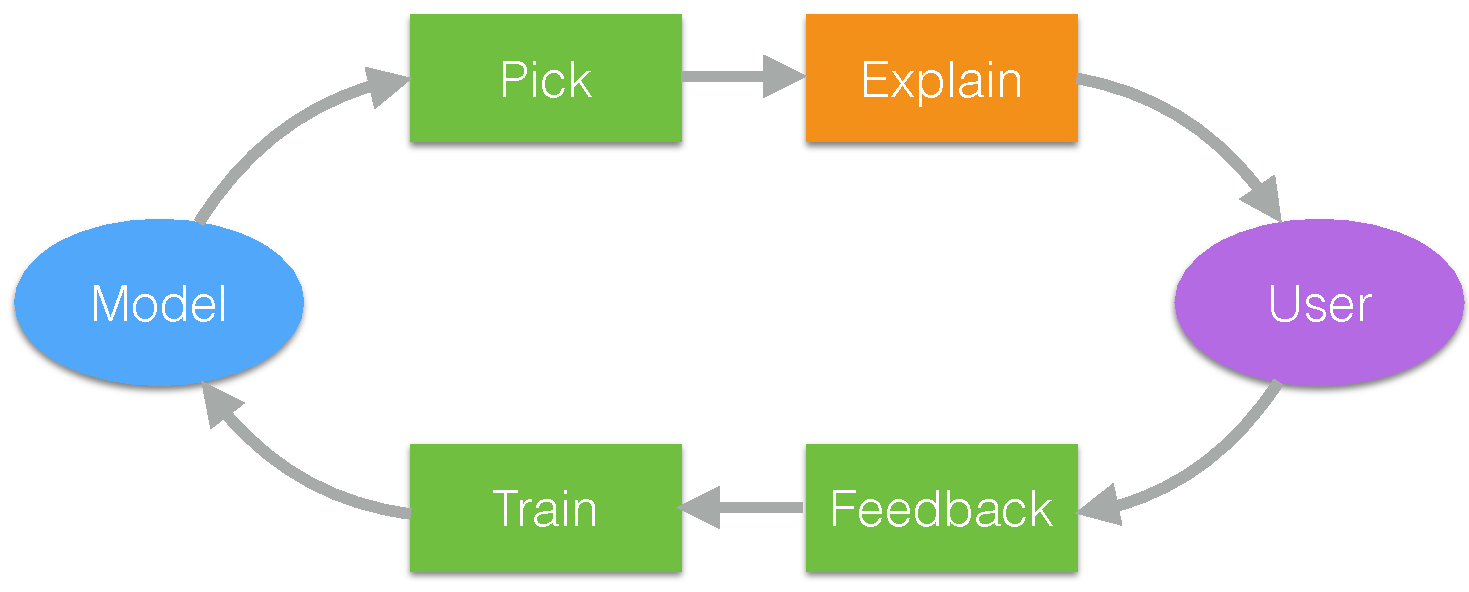
\includegraphics[width=.5\textwidth]{feedback_loop_cropped.pdf}
\caption{Machine learning loop}
\label{hmloop}
\end{figure}

The critical part in the loop where visualization comes is the \emph{explain}
box. This involves giving an overview of what the models are learning, as well
as explaining individual predictions. This is the primary focus of this work -
along with a simple mechanism for \textbf{feedback}, which is required if we are
to have a full loop. We focus primarily on text data, and on the multi-class
classification task. For simplicity, we assume that the bag-of-words
representation is used, although we plan on relaxing this assumption in future
work, as our visualizations generally do not depend on it.

Our tool has three top ``views'', which share a common visualization underneath
that allows the users to interact with the dataset. The first view is meant to explain
individual predictions to users, in terms of feature contributions. The second
view gives the users a global ``summary'' of the model, in the form of summary
statistics and an interactive confusion matrix. Finally, the third view allows
the user to give feedback to the model. The kind of feedback we allow currently
concerns mainly data cleaning - which we argue is already important enough to
significantly improve most text classifiers.


\section{Literature Review}
The statement that understanding what machine learning models are really
learning leads to better models is not very controversial.  Patel et al
\cite{Patel:2008:ISM:1357054.1357160} conducted interviews with machine learning
/ HCI practitioners, and found a consensus regarding the following: (1) the
machine learning process is iterative and exploratory, (2) understanding data
and algorithms is really important, and (3) evaluation is hard and critical.
They do a study where they observe people trying to produce a digit classifier,
where they found that a lot of time people get stuck in part of the process
(e.g. model selection) when the problem is somewhere else (such as lack of
labeled data, or noise in the data). They also found that just looking at
summary statistics in cross validation (CV) data is not enough for evaluation -
all of the participants overestimated their models’ accuracy, when compared to a
hidden test set, due to CV quirks. This led the authors to produce Gestalt
\cite{gestalt}, a system aimed at software developers that exposes the Machine
Learning pipeline in steps. One can see a particular example all the way through
the pipeline, implement his own visualization, click on a confusion table to see
misclassified examples and click on an example and see the features or the raw
data. Unfortunately, no explanation of how the model is interacting with the
data is provided to the user, so it may be hard to determine what to do to
improve the model.

On a similar line of research, \cite{modeltracker} provides a
visualization where examples are sorted according to the model's prediction, and
colored by their true class (which was the inspiration for our databin
visualization). You can click on an example to see the raw data. Any interaction
(adding features, relabeling examples, etc) which makes an example move produces
an arrow from the previous position to the next position. Their visualizations
are helpful, but there is no support for multi-class classification, or
explanation of why the model is making predictions the way it is. Also, the
visualization does not scale to larger datasets, as there is not enough space in
the screen for all of the points.

Some research has been done on explaining individual predictions, or giving an
overall explanation for the model. In \cite{explain:krr15}, the authors
``distill'' a matrix factorization model into rules (trying to be faithful to
the original model, while being more interpretable). It is unclear as to how
helpful these are, as there is still a problem of selecting which rules to show
to the user. In \cite{Strumbelj:2010:EEI:1756006.1756007}, the authors focus on
explaining individual classifications by highlighting individual feature
contributions, taking into account the interactions between features. Contrary
to the name, their method is not efficient at all, as it takes over an hour to
generate an explanation for an individual prediction in a dataset with 279
features (which is very modest for today's standards), so it could not be used
for interactive visualization.

More in line with our vision of machine learning as a loop,
\cite{Stumpf:2009:IMM:1555003.1555106} did an experiment where the system
explained itself to the user by showing rules, Na\"{i}ve Bayes ``weights'' or
similar examples to the one being classified. The users then provided free form
feedback (on paper), which they later tried to incorporate retroactively. Both
their explanations and some of their feedback are model-dependent, working only
with Na\"{i}ve Bayes. In fact, in follow up work
\cite{Kulesza:2011:WED:2030365.2030367} they develop an interactive system
focused only on Na\"{i}ve Bayes, where the explanation is guided by user questions,
such as ``why is this example classified positive''. One drawback of their
system is that feedback is very limited (just relabeling documents), and it's
not clear how useful it is - in fact it seems that it usually harms the
system's performance. It is also not very interactive, which is a feature that
most participants in their study really wanted - being able to change something
and seeing the results right away. 

Our main contributions are combining all of the following in one system: (1)
treating the process as a loop and allowing for feedback, (2) explaining individual
predictions - visually and interactively, (3) allowing for multiclass
classification, (4) interactivity in both the individual prediction explanations
and ``global'' model explanations, (5) handling larger datasets (to a certain
extent), and (6) being model-agnostic - i.e. working with any machine learning
classification model.

\section{The Backend, Feature Importance}

\section{The Databin}
\begin{figure}
  \subfloat[Likelihood binning]{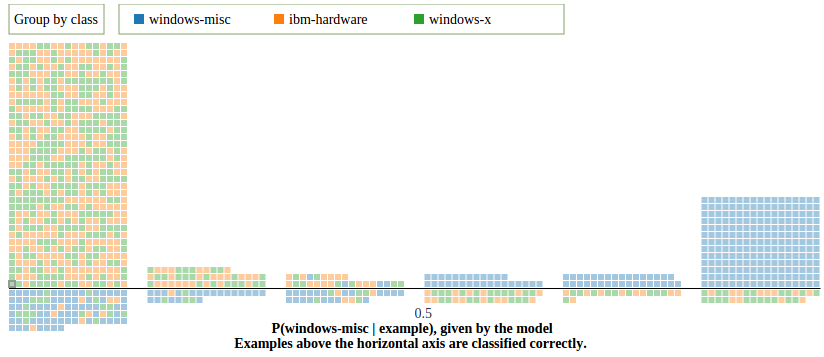
\includegraphics[width=.5\textwidth]{likelihood_bin}}\\
  \subfloat[Class binning]{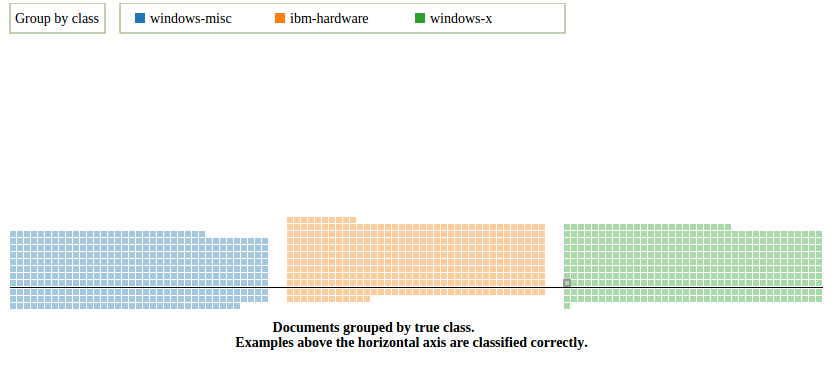
\includegraphics[width=.5\textwidth]{class_bin}}
  \caption{Two databin modes}
  \label{fig:databin}
\end{figure}

The main tool we use for visualizing a dataset as a whole is the
\textit{databin} (see Figure~\ref{fig:databin}). With this visualization, the
user is given an overview of how the model classifies each document. In
addition, the databin is interactive, and allows users to examine certain
documents by clicking on them, or seeing more information about an example by
hovering over it. With the encodings we've chosen, it is immediately evident
what documents the model may be overfitting on, thereby speeding up the Explain
and Feedback steps.

This visualization is similar to and inspired by \cite{modeltracker}, but with
several notable changes. A major limitation of Modeltracker is that it cannot
handle more than two classes, but most non-trivial machine learning
classification problems consist of multiple classes. Hence, we've used different
encodings and interactions in order to represent the performance on multiple
classes in a two-dimensional space. In addition, in contrast to the positional
encodings used by Modeltracker and our initial databin mode (\textit{likelihood
binning}), we've added an additional mode (which we call \textit{class
binning}). In this mode, examples can be binned by class instead of their model
likelihood. 

\textbf{Likelihood binning} In this mode, each example $x_i$ is represented with
a single square whose color is determined by the true class of the example $y_i$
We encode the likelihood $p(y\ |\ x_i)$ of an example $x_i$ belonging to a
particular class $y$ with the horizontal bin of the square. The class $y$
can be changed by clicking on the corresponding legend entry, and any changes
are animated. We use the vertical position to encode whether or not an example
was classified correctly. All examples whose true class $y_i$ equals the model's
prediction $y$ are binned above the horizontal line, and vice versa for
mistakes. This makes it very simple to see which examples the model has
classified incorrectly. For instance, the model is very confident on examples at
either extreme of the horizontal. If there exist some examples below the
horizontal line at these extremes, then the model has made a very confident
mistake, which is usually indicitive of some underlying problem that needs to be
rectified by a user.

\textbf{Class binning} We can use an alternative horizontal encoding to see the
performance on all classes in parallel. Instead of using the likelihood to
encode which bin an example, we simply bin each class separately. We still use
the same vertical and color encodings. In this mode, it is simple to see if a
model is underperforming on one class in particular.


\section{Explaining individual predictions}
\section{Global statistics}
\begin{figure}
  \subfloat[Cells in the confusion matrix are
  interactive]{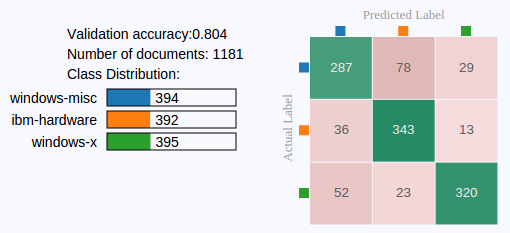
\includegraphics[width=.5\textwidth]{statistics}}\\
  \subfloat[When a cell is clicked, the corresponding examples are
  brushed]{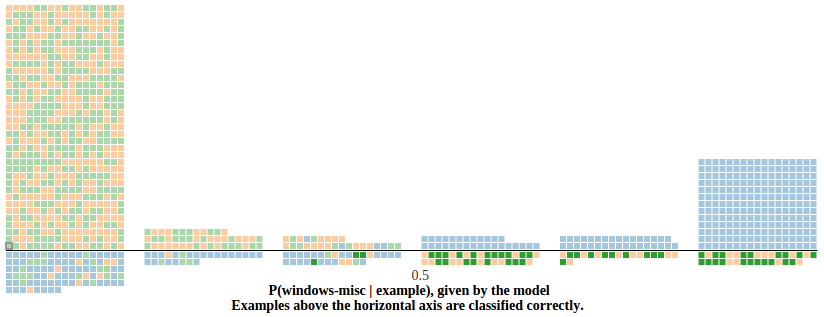
\includegraphics[width=.5\textwidth]{statistics_brush}}
  \caption{The global statistics visualization.}
  \label{fig:statistics}
\end{figure}

If the user wants a more quantitative view of the model performance, they can
select the ``Global Statistics'' tab, which includes standard metrics such as
accuracy and the label distributions. In addition, an interactive confusion
matrix is included. The user can select one of the cells in the matrix, and the
corresponding entries are brushed in the databin (see
Figure~\ref{fig:statistics}). This aids the user in determining why a certain
example is classified as something other than its true label. For instance, it
may include an email address that is present in many other documents of a
separate class, which is an incorrect feature to apply high weight to.

\section{Feedback}
\section{Conclusions / Future work}

% \section{Page Size and Columns}
% 
% On each page your material (not including the page number) should fit
% within a rectangle of 18 x 23.5 cm (7 x 9.25 in.), centered on a US
% letter page, beginning 1.9 cm (.75 in.) from the top of the page, with
% a .85 cm (.33 in.) space between two 8.4 cm (3.3 in.) columns.  On an
% A4 page, use a text area of the same dimensions (18 x 23.5 cm.), again
% centered.  Right margins should be justified, not ragged. Beware,
% especially when using this template on a Macintosh, Word can change
% these dimensions in unexpected ways.
% 
% \section{Typeset Text}
% 
% Prepare your submissions on a word processor or typesetter.  Please
% note that page layout may change slightly depending upon the printer
% you have specified.  For this document, printing to Adobe Acrobat PDF
% Writer was specified.  In the resulting page layout, Figure 1 appears
% at the top of the left column on page 2, and Table 1 appears at the
% top of the right column on page 2.  You may need to reposition the
% figures if your page layout or PDF-generation software is different.
% 
% \subsection{Title and Authors}
% 
% Your paper's title, authors and affiliations should run across the
% full width of the page in a single column 17.8 cm (7 in.) wide.  The
% title should be in Helvetica 18-point bold; use Arial if Helvetica is
% not available.  Authors' names should be in Times Roman 12-point bold,
% and affiliations in Times Roman 12-point (note that Author and
% Affiliation are defined Styles in this template file).
% 
% To position names and addresses, use a single-row table with invisible
% borders, as in this document.  Alternatively, if only one address is
% needed, use a centered tab stop to center all name and address text on
% the page; for two addresses, use two centered tab stops, and so
% on. For more than three authors, you may have to place some address
% information in a footnote, or in a named section at the end of your
% paper. Please use full international addresses and telephone dialing
% prefixes.  Leave one 10-pt line of white space below the last line of
% affiliations.
% 
% \subsection{Abstract and Keywords}
% 
% Every submission should begin with an abstract of about 150 words,
% followed by a set of keywords. The abstract and keywords should be
% placed in the left column of the first page under the left half of the
% title. The abstract should be a concise statement of the problem,
% approach and conclusions of the work described.  It should clearly
% state the paper's contribution to the field of HCI.
% 
% The first set of keywords will be used to index the paper in the
% proceedings. The second set are used to catalogue the paper in the ACM
% Digital Library. The latter are entries from the ACM Classification
% System~\cite{acm_categories}.  In general, it should only be necessary
% to pick one or more of the H5 subcategories, see
% http://www.acm.org/class/1998/H.5.html
% 
% \subsection{Normal or Body Text}
% 
% Please use a 10-point Times Roman font or, if this is unavailable,
% another proportional font with serifs, as close as possible in
% appearance to Times Roman 10-point. The Press 10-point font available
% to users of Script is a good substitute for Times Roman. If Times
% Roman is not available, try the font named Computer Modern Roman. On a
% Macintosh, use the font named Times and not Times New Roman. Please
% use sans-serif or non-proportional fonts only for special purposes,
% such as headings or source code text.
% 
% \subsection{First Page Copyright Notice}
% 
% Leave 3 cm (1.25 in.) of blank space for the copyright notice at the
% bottom of the left column of the first page. In this template a
% floating text box will automatically generate the required space.
% 
% \subsection{Subsequent Pages}
% 
% On pages beyond the first, start at the top of the page and continue
% in double-column format.  The two columns on the last page should be
% of equal length.
% 
% \subsection{References and Citations}
% 
% Use a numbered list of references at the end of the article, ordered
% alphabetically by first author, and referenced by numbers in brackets
% [2,4,5,7]. For papers from conference proceedings, include the title
% of the paper and an abbreviated name of the conference (e.g., for
% Interact 2003 proceedings, use Proc. Interact 2003). Do not include
% the location of the conference or the exact date; do include the page
% numbers if available. See the examples of citations at the end of this
% document. Within this template file, use the References style for the
% text of your citation.
% 
% Your references should be published materials accessible to the
% public.  Internal technical reports may be cited only if they are
% easily accessible (i.e., you provide the address for obtaining the
% report within your citation) and may be obtained by any reader for a
% nominal fee.  Proprietary information may not be cited. Private
% communications should be acknowledged in the main text, not referenced
% (e.g., ``[Robertson, personal communication]'').


\bibliographystyle{abbrv}
\bibliography{sample}

\end{document}
